%=============================================================================
% Engineering Design Document
% ψ-Field Energy Harvester and Storage Module
%
% Patent #7: ψ-Field Energy Harvesting and Storage Systems
% Author: Gary Thomas Alcock
% Generated: 2026-03-19
%=============================================================================

\documentclass[11pt,a4paper]{article}

\usepackage{amsmath,amssymb}
\usepackage{physics}
\usepackage{siunitx}
\usepackage{graphicx}
\usepackage{booktabs}
\usepackage{longtable}
\usepackage{hyperref}
\usepackage{xcolor}
\usepackage{tikz}
\usepackage{pgfplots}
\pgfplotsset{compat=1.18}
\usetikzlibrary{patterns,arrows.meta,positioning,decorations.markings,shapes.geometric}
\usepackage[margin=2.5cm]{geometry}
\usepackage{fancyhdr}
\usepackage{tcolorbox}

\pagestyle{fancy}
\fancyhead[L]{\small Patent \#7 --- $\psi$-Field Energy Harvester}
\fancyhead[R]{\small DFD Engineering Design}
\fancyfoot[C]{\thepage}

\title{\Large\textbf{Engineering Design Document} \\[0.5em]
\large $\psi$-Field Energy Harvester and Storage Module \\[0.3em]
\normalsize Patent \#7: $\psi$-Field Energy Harvesting and Storage Systems}

\author{Gary Thomas Alcock \\
\small Density Field Dynamics Programme}

\date{March 2026 \\ \small Document Rev.\ 1.0}

\begin{document}
\maketitle
\tableofcontents
\newpage

%=============================================================================
\section{Executive Summary}
%=============================================================================

This document specifies the complete engineering design for a modular
$\psi$-field energy harvester and storage system based on Density Field
Dynamics (DFD).  The system exploits the electromagnetic--$\psi$ coupling
(parameterized by $\lambda$) to transfer energy bidirectionally between
superconducting RF cavity modes and standing $\psi$-wave configurations.

The design encompasses three configurations of increasing scale:

\begin{enumerate}
\item \textbf{Mark~I --- Detection Module:} Establishes whether
$|\lambda-1| \neq 0$.  No harvesting; pure measurement.  Uses existing
SRF infrastructure.

\item \textbf{Mark~II --- Proof-of-Concept Harvester:} Demonstrates
bidirectional EM$\leftrightarrow\psi$ energy transfer.  Measures
round-trip efficiency and mode characterization.

\item \textbf{Mark~III --- Scalable Storage Array:} Multi-module array
for practical energy storage.  Targets grid-scale and pulsed-power
applications.
\end{enumerate}

\begin{tcolorbox}[colback=red!5!white, colframe=red!60!black, title=Critical Dependency]
The entire system depends on $|\lambda-1| \neq 0$.  The Mark~I module
must confirm this before proceeding to Mark~II/III.  The current
accidental bound is $|\lambda-1| \lesssim 3\times 10^{-5}$.  The
Mark~I design achieves $|\lambda-1| \sim 10^{-14}$ sensitivity.
\end{tcolorbox}

%=============================================================================
\section{System Architecture}
%=============================================================================

\subsection{Functional Block Diagram}

The $\psi$-field harvester/storage module consists of five primary
subsystems:

\begin{enumerate}
\item \textbf{EM Cavity Subsystem:} Superconducting RF cavity providing
high-Q electromagnetic modes for pumping and extraction.

\item \textbf{$\psi$-Resonator Subsystem:} Physical enclosure with
$\psi$-reflective boundaries sustaining standing $\psi$-wave modes.

\item \textbf{Coupling Interface:} Region of spatial overlap between
EM and $\psi$ modes enabling parametric energy transfer.

\item \textbf{Control and Readout Electronics:} RF drive, modulation,
phase-sensitive detection, and feedback systems.

\item \textbf{Cryogenic Infrastructure:} Liquid helium cooling for
superconducting cavity operation.
\end{enumerate}

\begin{figure}[h]
\centering
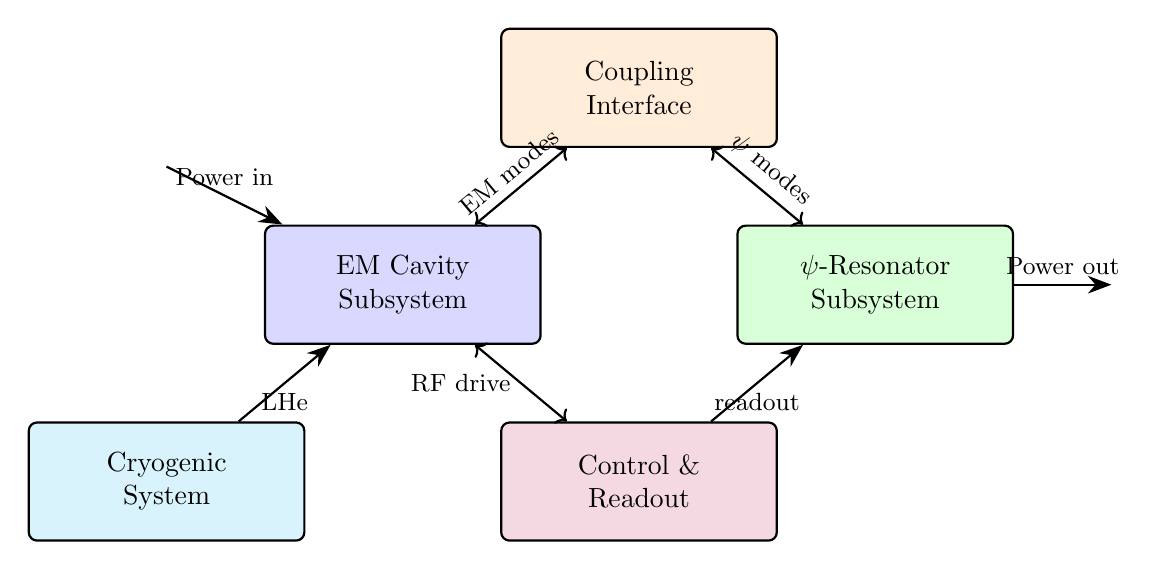
\begin{tikzpicture}[
  block/.style={draw, thick, minimum width=3.5cm, minimum height=1.5cm,
    align=center, rounded corners=3pt},
  arrow/.style={-{Stealth[length=3mm]}, thick}
]

% Blocks
\node[block, fill=blue!15] (em) at (0,0) {EM Cavity\\Subsystem};
\node[block, fill=green!15] (psi) at (6,0) {$\psi$-Resonator\\Subsystem};
\node[block, fill=orange!15] (couple) at (3,2.5) {Coupling\\Interface};
\node[block, fill=purple!15] (ctrl) at (3,-2.5) {Control \&\\Readout};
\node[block, fill=cyan!15] (cryo) at (-3,-2.5) {Cryogenic\\System};

% Arrows
\draw[arrow, <->] (em) -- node[above, sloped, font=\small] {EM modes} (couple);
\draw[arrow, <->] (psi) -- node[above, sloped, font=\small] {$\psi$ modes} (couple);
\draw[arrow, <->] (em) -- node[left, font=\small] {RF drive} (ctrl);
\draw[arrow] (ctrl) -- node[below, font=\small] {readout} (psi);
\draw[arrow] (cryo) -- node[below, font=\small] {LHe} (em);

% External
\draw[arrow] (-3, 1.5) -- node[above, font=\small] {Power in} (em);
\draw[arrow] (psi) -- node[above, font=\small] {Power out} (9, 0);

\end{tikzpicture}
\caption{Functional block diagram of the $\psi$-field harvester/storage module.}
\label{fig:block}
\end{figure}

\subsection{Operating Modes}

\begin{table}[h]
\centering
\caption{System operating modes.}
\label{tab:modes}
\begin{tabular}{@{}llll@{}}
\toprule
Mode & Direction & EM state & $\psi$ state \\
\midrule
Detection & --- & Driven at $\omega$, modulated at $2\omega$ & Monitored \\
Charging & EM $\to$ $\psi$ & Driven, parametric pump & Amplitude grows \\
Storage & Hold & Off (or low-level maintenance) & Free decay \\
Discharge & $\psi$ $\to$ EM & Seed mode, parametric extract & Amplitude decays \\
Standby & --- & Off & Off \\
\bottomrule
\end{tabular}
\end{table}

%=============================================================================
\section{Mark~I: Detection Module}
%=============================================================================

\subsection{Purpose}

Detect or constrain $|\lambda-1|$ to the $10^{-14}$ level using the
EM--$\psi$ parametric coupling protocol.  This is the go/no-go gate for
the entire program.

\subsection{Design Philosophy}

Maximize sensitivity by:
\begin{itemize}
\item Using an existing high-performance SRF cavity (e.g., DESY/XFEL
or FNAL type, 1.3~GHz 9-cell niobium)
\item Operating in TE+TM superposition to restore the driven overlap $G$
\item Applying deliberate $2\omega$ amplitude modulation with $m = 0.1$
\item Preserving (not suppressing) $2\omega$ response in readout
\end{itemize}

\subsection{Technical Specifications}

\begin{longtable}{@{}p{6cm}p{8cm}@{}}
\caption{Mark~I Detection Module --- Specifications.} \label{tab:mk1} \\
\toprule
\textbf{Parameter} & \textbf{Value} \\
\midrule
\endfirsthead
\toprule
\textbf{Parameter} & \textbf{Value} \\
\midrule
\endhead
\bottomrule
\endfoot
\multicolumn{2}{l}{\textit{EM Cavity}} \\
\midrule
Cavity type & Niobium SRF, TESLA-type 9-cell \\
Operating frequency & 1.3~GHz (TM$_{010}$ $\pi$-mode) \\
Secondary mode & TE$_{011}$ at nearby frequency \\
Intrinsic $Q_0$ & $> 2\times 10^{10}$ (N-doped) \\
Stored energy & $U_0 = 100$~kJ (pulsed, $E_{\rm acc} \approx 25$~MV/m) \\
Operating temperature & 2.0~K \\
Cavity length & 1.038~m (active length) \\
Cavity aperture & $70$~mm iris diameter \\
\midrule
\multicolumn{2}{l}{\textit{$\psi$-Mode Geometry}} \\
\midrule
$\psi$-tube length $L$ & 1.0~m (defined by end-cap spacing) \\
$\psi$-tube cross-section $A_\psi$ & 0.80~m$^2$ (cryostat bore) \\
End-cap material & Tungsten alloy (W-25Re), $\rho = 19\,700$~kg/m$^3$ \\
End-cap thickness & 100~mm \\
Fundamental $\psi$-frequency & $f_\psi = c_s/(2L) \approx 150$~MHz (for $c_s = c$) \\
Estimated $Q_\psi$ & $> 10^3$ (conservative) \\
Total cavity aperture $A_{\rm cav,tot}$ & $3\times 10^{-2}$~m$^2$ (9 irises) \\
\midrule
\multicolumn{2}{l}{\textit{Modulation and Readout}} \\
\midrule
Modulation frequency & $2\omega_{\rm EM} = 2.6$~GHz \\
Modulation depth $m$ & 0.1 (on stored energy envelope) \\
Modulation method & Amplitude modulation via klystron drive \\
Readout method & Phase-sensitive detection at $\Omega_\psi$ \\
Readout sensitivity target & $\Delta\psi \leq 10^{-14}$ \\
Signal integration time & Up to $10^4$~s per run \\
\midrule
\multicolumn{2}{l}{\textit{TE+TM Superposition}} \\
\midrule
Mode combination & TM$_{010}$ + TE$_{011}$ co-phased \\
Overlap parameter $\eta_\times$ & $\sim 0.3$ (estimated) \\
Relative phase $\phi$ & 0 (maximizes $G$) \\
Phase stability requirement & $\delta\phi < 0.01$~rad \\
\midrule
\multicolumn{2}{l}{\textit{Sensitivity Projections}} \\
\midrule
Accidental bound (existing) & $|\lambda-1| \lesssim 3\times 10^{-5}$ \\
Design sensitivity (parametric) & $|\lambda-1|_{\rm min} \sim 10^{-14}$ \\
Design sensitivity (driven) & $\Delta\psi \sim 1.2\times 10^{-3}|\lambda-1|$ \\
\midrule
\multicolumn{2}{l}{\textit{Physical Envelope}} \\
\midrule
Cryostat outer diameter & 1.5~m \\
Total assembly length & 3.0~m (cavity + end-caps + services) \\
Total mass & $\approx 3500$~kg (incl.\ cryostat, shields) \\
Cryogenic load & $\sim 10$~W at 2~K \\
RF power (peak) & $\sim 200$~kW (klystron) \\
\end{longtable}

\subsection{Detection Protocol}

\begin{enumerate}
\item \textbf{Baseline calibration:} Operate cavity in TM$_{010}$ alone.
Record noise floor at $\Omega_\psi$ with $2\omega$ modulation.  This
establishes the null (no driven overlap, $G \approx 0$).

\item \textbf{TE+TM measurement:} Activate TE$_{011}$ mode simultaneously.
Phase-lock to TM$_{010}$.  Monitor readout at $\Omega_\psi$.

\item \textbf{Modulation sweep:} Vary $2\omega$ across the expected
$\psi$-mode bandwidth ($\Delta\Omega_\psi/\Omega_\psi \sim Q_\psi^{-1}$).
Search for resonant enhancement.

\item \textbf{Confirmation:} Repeat with $\phi = \pi/2$ (should null
the signal).  Vary $m$ and verify linear scaling.  Change end-cap
spacing and verify frequency shift.
\end{enumerate}

\subsection{Signal Signatures}

A positive detection would show:
\begin{itemize}
\item Resonant peak at $\Omega_\psi = n\pi c_s/L$ in phase-sensitive readout
\item Linear scaling with modulation depth $m$
\item Quadratic scaling with stored energy $U_0$
\item Nulling when $\phi = \pi/2$
\item Frequency shift proportional to $1/L$ when end-cap spacing is changed
\item Exponential growth above parametric threshold
\end{itemize}

%=============================================================================
\section{Mark~II: Proof-of-Concept Harvester}
%=============================================================================

\subsection{Purpose}

Demonstrate bidirectional energy transfer between EM and $\psi$ modes.
Measure round-trip efficiency.  Characterize the $\psi$-mode spectrum
and quality factors.

\subsection{Design Modifications from Mark~I}

\begin{itemize}
\item Optimized coupling geometry (cavity at $\psi$-mode antinodes)
\item Higher stored energy capability ($U_0$ up to 1~MJ pulsed)
\item Dedicated extraction antenna and impedance-matching network
\item Programmable mode-switching for charge/discharge cycling
\item Calorimetric measurement system for energy accounting
\end{itemize}

\subsection{Technical Specifications}

\begin{longtable}{@{}p{6cm}p{8cm}@{}}
\caption{Mark~II PoC Harvester --- Key specifications beyond Mark~I.}
\label{tab:mk2} \\
\toprule
\textbf{Parameter} & \textbf{Value} \\
\midrule
\endfirsthead
\toprule
\textbf{Parameter} & \textbf{Value} \\
\midrule
\endhead
\bottomrule
\endfoot
\multicolumn{2}{l}{\textit{Enhanced EM System}} \\
\midrule
Maximum stored energy & 1~MJ (pulsed, $E_{\rm acc} \approx 45$~MV/m) \\
Pulse repetition rate & 1--10~Hz \\
Extraction antenna $Q_{\rm ext}$ & Adjustable $10^3$--$10^{10}$ \\
Impedance matching & Programmable stub tuner, $< 50$~ns switching \\
\midrule
\multicolumn{2}{l}{\textit{Optimized $\psi$-Resonator}} \\
\midrule
Tube cross-section $A_\psi$ & 0.27~m$^2$ (reduced for higher $H$) \\
Multiple cavity placement & 3 cavities at $\psi$-mode antinodes \\
Total cavity aperture & $0.09$~m$^2$ \\
$\psi$-mode quality target & $Q_\psi > 10^4$ \\
\midrule
\multicolumn{2}{l}{\textit{Energy Accounting}} \\
\midrule
Input power meter & Directional coupler, $\pm 0.1\%$ \\
Output power meter & Calibrated load, calorimetric \\
$\psi$-mode energy estimate & From cavity detuning measurement \\
Round-trip efficiency target & $> 10\%$ (first demonstration) \\
\midrule
\multicolumn{2}{l}{\textit{Charge/Discharge Cycle}} \\
\midrule
Charge time (projected) & 1--100~$\mu$s \\
Storage time (hold) & 1~$\mu$s--1~ms \\
Discharge time & 1--100~$\mu$s \\
Cycle repetition & Up to $10^3$~Hz \\
\midrule
\multicolumn{2}{l}{\textit{Physical Envelope}} \\
\midrule
Total assembly length & 5.0~m \\
Cryostat outer diameter & 2.0~m \\
Total mass & $\approx 8000$~kg \\
Floor space & 3~m $\times$ 8~m (incl.\ services) \\
\end{longtable}

\subsection{Measurement Program}

\begin{enumerate}
\item \textbf{$\psi$-mode spectroscopy:}
  \begin{itemize}
  \item Sweep EM modulation frequency across $50$--$500$~MHz
  \item Map all accessible $\psi$-modes up to $n = 5$
  \item Extract $c_s$ from mode spacing: $c_s = 2L\Delta f$
  \item Measure $Q_\psi$ from ringdown: drive $\psi$-mode, cut EM drive,
    observe exponential decay
  \end{itemize}

\item \textbf{Bidirectional transfer demonstration:}
  \begin{itemize}
  \item Charge: Pump $\psi$-mode with EM energy, measure transfer rate
  \item Hold: Turn off EM, measure $\psi$-mode decay time
  \item Extract: Reactivate EM cavity, measure energy returned
  \item Accounting: Compare input, stored, and output energies
  \end{itemize}

\item \textbf{Efficiency optimization:}
  \begin{itemize}
  \item Vary modulation depth $m$: $0.01$--$0.3$
  \item Vary extraction $Q_{\rm ext}$: optimize impedance matching
  \item Vary cavity placement: test antinode vs.\ node positioning
  \item Thermal management: characterize heat load vs.\ cycle rate
  \end{itemize}
\end{enumerate}

%=============================================================================
\section{Mark~III: Scalable Storage Array}
%=============================================================================

\subsection{Purpose}

Demonstrate a practical energy storage system using an array of
$\psi$-resonator modules.  Target applications: pulsed power,
grid frequency regulation, directed energy.

\subsection{Module Design}

Each Mark~III module is an optimized, compact version of the Mark~II
proof-of-concept system.

\begin{longtable}{@{}p{6cm}p{8cm}@{}}
\caption{Mark~III Storage Module --- Specifications.}
\label{tab:mk3} \\
\toprule
\textbf{Parameter} & \textbf{Value} \\
\midrule
\endfirsthead
\toprule
\textbf{Parameter} & \textbf{Value} \\
\midrule
\endhead
\bottomrule
\endfoot
\multicolumn{2}{l}{\textit{Individual Module}} \\
\midrule
Module dimensions & 0.5~m dia.\ $\times$ 2.0~m length \\
Module mass & $\sim 800$~kg (incl.\ cryostat) \\
EM cavity & Nb$_3$Sn coated, $Q_0 > 10^{11}$, 4.2~K operation \\
Stored EM energy & 100~kJ per module \\
$\psi$-mode storage energy & Depends on $|\lambda-1|$ and $q_{\rm max}$ \\
Target storage (at $q_{\rm max} = 10^{-10}$) & $\sim 2$~GJ per module \\
Discharge time & $1$--$100~\mu$s \\
Peak discharge power & $\sim 20$~GW per module \\
Round-trip efficiency target & $> 70\%$ \\
Operating temperature & 4.2~K (Nb$_3$Sn allows higher $T$) \\
\midrule
\multicolumn{2}{l}{\textit{Array Configuration}} \\
\midrule
Modules per rack & 8 (vertical stack) \\
Rack dimensions & 1.0~m $\times$ 1.0~m $\times$ 4.5~m height \\
Racks per array & 10 \\
Total modules & 80 \\
Total storage energy & $\sim 160$~GJ ($\sim 44$~MWh) \\
Total peak power & $\sim 1.6$~TW \\
Array footprint & $10$~m $\times$ 5~m \\
Shared cryogenic plant & 500~W at 4.2~K \\
\midrule
\multicolumn{2}{l}{\textit{Control and Power Electronics}} \\
\midrule
RF source per module & Solid-state amplifier, 50~kW CW \\
Modulation control & FPGA-based, $< 10$~ns timing \\
Array sequencer & Central controller, fiber-optic links \\
Output power conditioning & Marx bank or pulse-forming network \\
Grid interface (if applicable) & 3-phase inverter, 10~MVA \\
\end{longtable}

\subsection{Array Architecture}

\begin{figure}[h]
\centering
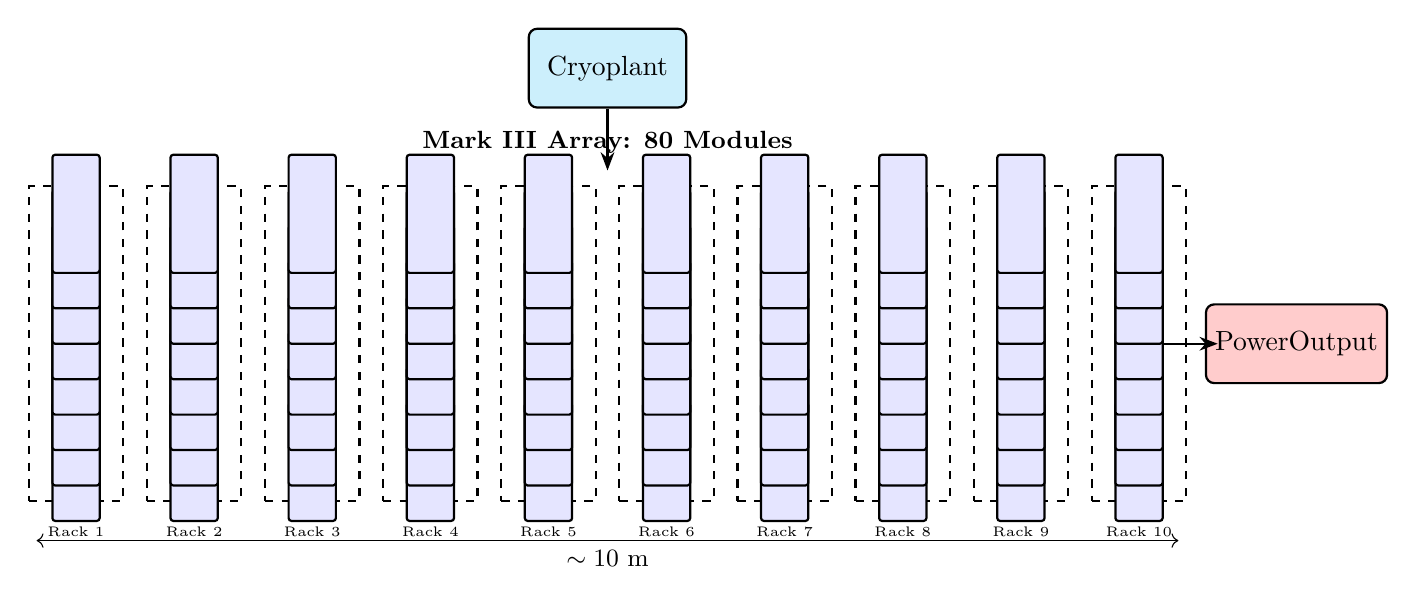
\begin{tikzpicture}[
  module/.style={draw, thick, fill=blue!10, minimum width=0.6cm,
    minimum height=1.5cm, rounded corners=1pt},
  rack/.style={draw, thick, dashed, minimum width=1.2cm, minimum height=4cm}
]

% Draw 10 racks, each with 8 modules
\foreach \r in {0,...,9} {
  \node[rack] (rack\r) at (1.5*\r, 0) {};
  \foreach \m in {0,...,7} {
    \node[module] at (1.5*\r, -1.5+0.45*\m) {};
  }
  \node[below, font=\tiny] at (1.5*\r, -2.2) {Rack \the\numexpr\r+1};
}

% Labels
\node[above, font=\small\bfseries] at (6.75, 2.3) {Mark~III Array: 80 Modules};
\draw[<->] (-0.5, -2.5) -- (14, -2.5) node[midway, below, font=\small] {$\sim 10$~m};

% Shared cryoplant
\node[draw, thick, fill=cyan!20, minimum width=2cm, minimum height=1cm,
  rounded corners=3pt] (cryo) at (6.75, 3.5) {Cryoplant};
\draw[thick, -{Stealth}] (cryo) -- (6.75, 2.2);

% Power output
\node[draw, thick, fill=red!20, minimum width=2cm, minimum height=1cm,
  rounded corners=3pt] (power) at (15.5, 0) {Power\\Output};
\draw[thick, -{Stealth}] (13.8, 0) -- (14.5, 0);

\end{tikzpicture}
\caption{Mark~III array layout: 10 racks of 8 modules each, with shared
  cryogenic plant and centralized power output.}
\label{fig:array}
\end{figure}

\subsection{Operating Scenarios}

\subsubsection{Scenario A: Grid Frequency Regulation}

\begin{itemize}
\item \textbf{Mode:} Continuous charge/discharge at grid frequency
  deviations.
\item \textbf{Response time:} $< 1$~ms (limited by power electronics,
  not $\psi$-mode dynamics).
\item \textbf{Energy per cycle:} $\sim 1$~MJ (partial charge/discharge).
\item \textbf{Cycle rate:} Up to 100~Hz.
\item \textbf{Continuous power:} $\sim 100$~MW.
\item \textbf{Duration:} Indefinite (continuous cycling, net energy from
  grid or renewable source).
\end{itemize}

\subsubsection{Scenario B: Pulsed Power}

\begin{itemize}
\item \textbf{Mode:} Slow charge (minutes), fast discharge ($\mu$s).
\item \textbf{Charge source:} Grid or dedicated generator.
\item \textbf{Peak power:} $\sim 1.6$~TW (all 80 modules simultaneous).
\item \textbf{Pulse energy:} Up to 160~GJ.
\item \textbf{Pulse duration:} $1$--$100~\mu$s.
\item \textbf{Repetition:} Limited by recharge time (minutes).
\end{itemize}

\subsubsection{Scenario C: Renewable Integration}

\begin{itemize}
\item \textbf{Mode:} Buffer for solar/wind variability.
\item \textbf{Charge:} During surplus generation.
\item \textbf{Discharge:} During shortfall.
\item \textbf{Total energy:} $\sim 44$~MWh.
\item \textbf{Round-trip efficiency:} $> 70\%$.
\item \textbf{Footprint advantage:} $\sim 50$~m$^2$ vs.\ $\sim 5000$~m$^2$
  for equivalent Li-ion installation.
\end{itemize}

%=============================================================================
\section{Subsystem Detailed Design}
%=============================================================================

\subsection{EM Cavity Subsystem}

\subsubsection{Cavity Selection}

The baseline cavity is a TESLA-type 9-cell niobium structure operating
at 1.3~GHz in the TM$_{010}$ $\pi$-mode.  This choice leverages decades
of SRF cavity R\&D and an extensive industrial supply chain.

Key modifications for $\psi$-harvesting:
\begin{itemize}
\item \textbf{TE$_{011}$ port:} Additional coupling port optimized for
TE$_{011}$ excitation, positioned to maximize overlap with TM$_{010}$.
\item \textbf{Phase-locked loop:} Dual-mode PLL maintaining relative
phase $\phi$ between TE and TM modes to $< 0.01$~rad.
\item \textbf{$2\omega$ modulation:} Direct amplitude modulation of the
klystron drive at $2\times 1.3 = 2.6$~GHz.
\end{itemize}

\subsubsection{Cavity Performance Budget}

\begin{table}[h]
\centering
\caption{EM cavity performance budget.}
\label{tab:cavity-budget}
\begin{tabular}{@{}lcc@{}}
\toprule
Parameter & Mark~I & Mark~III \\
\midrule
Cavity material & Nb (bulk) & Nb$_3$Sn on Cu \\
Operating $T$ (K) & 2.0 & 4.2 \\
$Q_0$ & $2\times 10^{10}$ & $10^{11}$ \\
$E_{\rm acc}$ (MV/m) & 25 & 25 \\
$U_0$ (kJ) & 100 & 100 \\
Dissipated power (W) & 5.3 & 1.1 \\
Fill time at $Q_L = 10^7$ (ms) & 2.4 & 2.4 \\
Bandwidth at $Q_L = 10^7$ (Hz) & 130 & 130 \\
\bottomrule
\end{tabular}
\end{table}

\subsection{$\psi$-Resonator Subsystem}

\subsubsection{Boundary Design}

The $\psi$-reflective boundaries are dense material end-caps.  The
reflection coefficient at a density discontinuity is:
\begin{equation}
|r_\psi|^2 \approx 1 - \frac{4\bar{\rho}}{\rho_{\rm cap}},
\end{equation}
where $\bar{\rho}$ is the cosmological mean density and $\rho_{\rm cap}$
is the end-cap density.

\begin{table}[h]
\centering
\caption{Candidate end-cap materials.}
\label{tab:endcap}
\begin{tabular}{@{}lccc@{}}
\toprule
Material & Density (kg/m$^3$) & $1 - |r_\psi|^2$ & Notes \\
\midrule
Lead & 11\,340 & $\sim 10^{-30}$ & Easy to machine \\
Tungsten & 19\,300 & $\sim 10^{-30}$ & Highest density metal \\
W-25Re alloy & 19\,700 & $\sim 10^{-30}$ & Better machinability \\
Depleted uranium & 19\,100 & $\sim 10^{-30}$ & Regulatory burden \\
Osmium & 22\,590 & $\sim 10^{-30}$ & Highest element density \\
\bottomrule
\end{tabular}
\end{table}

All candidate materials provide essentially perfect $\psi$-reflection.
The choice is driven by practical considerations: cost, machinability,
and compatibility with the cryogenic environment.  Tungsten alloy
(W-25Re) is the baseline choice.

\subsubsection{Resonator Geometry}

\begin{figure}[h]
\centering
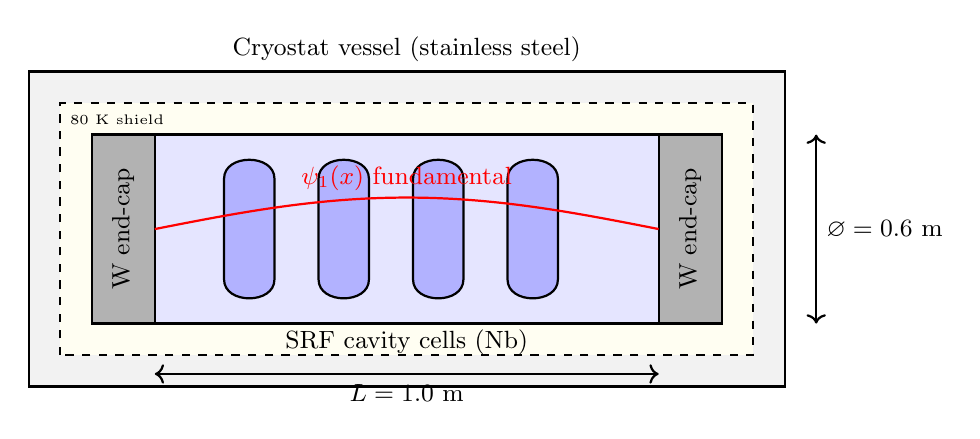
\begin{tikzpicture}[scale=0.8]

% Outer cryostat
\draw[thick, fill=gray!10] (-1, -2.5) rectangle (11, 2.5);
\node[above, font=\small] at (5, 2.5) {Cryostat vessel (stainless steel)};

% Thermal shields
\draw[thick, dashed, fill=yellow!5] (-0.5, -2.0) rectangle (10.5, 2.0);
\node[above right, font=\tiny] at (-0.5, 1.5) {80~K shield};

% Tungsten end-caps
\draw[thick, fill=gray!60] (0, -1.5) rectangle (1, 1.5);
\draw[thick, fill=gray!60] (9, -1.5) rectangle (10, 1.5);
\node[font=\small, rotate=90] at (0.5, 0) {W end-cap};
\node[font=\small, rotate=90] at (9.5, 0) {W end-cap};

% Cavity region
\draw[thick, fill=blue!10] (1, -1.5) rectangle (9, 1.5);

% SRF cavity (simplified)
\foreach \x in {2.5, 4, 5.5, 7} {
  \draw[thick, fill=blue!30] (\x-0.4, -0.8) .. controls (\x-0.4, -1.2) and (\x+0.4, -1.2) .. (\x+0.4, -0.8)
    -- (\x+0.4, 0.8) .. controls (\x+0.4, 1.2) and (\x-0.4, 1.2) .. (\x-0.4, 0.8) -- cycle;
}
\node[font=\small] at (5, -1.8) {SRF cavity cells (Nb)};

% Psi standing wave
\draw[thick, red, domain=1:9, samples=100] plot (\x, {0.5*sin((\x-1)*180/8)});
\node[font=\small, red] at (5, 0.8) {$\psi_1(x)$ fundamental};

% Dimensions
\draw[<->, thick] (1, -2.3) -- (9, -2.3) node[midway, below, font=\small] {$L = 1.0$~m};
\draw[<->, thick] (11.5, -1.5) -- (11.5, 1.5) node[midway, right, font=\small] {$\varnothing = 0.6$~m};

\end{tikzpicture}
\caption{Cross-section of the $\psi$-resonator assembly showing
  tungsten end-caps, SRF cavity cells, and fundamental $\psi$-mode
  standing wave.}
\label{fig:resonator}
\end{figure}

\subsubsection{$\psi$-Mode Spectrum}

For a cylindrical resonator of length $L$ and radius $R$ with perfectly
reflecting end-caps, the mode frequencies are:
\begin{equation}
f_{nmk} = \frac{c_s}{2\pi}\sqrt{\left(\frac{n\pi}{L}\right)^2 + \left(\frac{j_{mk}}{R}\right)^2},
\end{equation}
where $j_{mk}$ is the $k$-th zero of $J_m'$.

For $L = 1$~m, $R = 0.3$~m, $c_s = c$:

\begin{table}[h]
\centering
\caption{First five $\psi$-mode frequencies (axial modes, $m=k=0$).}
\label{tab:psi-modes}
\begin{tabular}{@{}cccc@{}}
\toprule
$n$ & $f_n$ (MHz) & $\Omega_n$ (Grad/s) & $\lambda_n$ (m) \\
\midrule
1 & 150 & 0.94 & 2.0 \\
2 & 300 & 1.88 & 1.0 \\
3 & 450 & 2.83 & 0.67 \\
4 & 600 & 3.77 & 0.50 \\
5 & 750 & 4.71 & 0.40 \\
\bottomrule
\end{tabular}
\end{table}

\subsection{Control and Readout Electronics}

\subsubsection{RF Drive Chain}

\begin{enumerate}
\item \textbf{Master oscillator:} Ultra-stable crystal oscillator at
1.3~GHz, phase noise $< -150$~dBc/Hz at 1~kHz offset.

\item \textbf{$2\omega$ modulator:} Direct digital synthesis of 2.6~GHz
modulation tone, locked to master oscillator.  Variable depth $m = 0$--$0.3$.

\item \textbf{Power amplifier:} Klystron (Mark~I/II) or solid-state
(Mark~III), 50--200~kW peak.

\item \textbf{Circulator and load:} Protect amplifier from reflected
power.  Directional couplers for power measurement.

\item \textbf{TE mode coupler:} Separate port with independent phase
control for TE$_{011}$ excitation.
\end{enumerate}

\subsubsection{$\psi$-Mode Readout}

The $\psi$-mode amplitude modulates the EM cavity resonant frequency
through the constitutive relation $\varepsilon_{\rm eff}(\psi)$.  This
produces sidebands on the cavity transmission at $\pm\Omega_\psi$ from
the carrier.

\begin{enumerate}
\item \textbf{Phase-sensitive detector:} Lock-in amplifier referenced to
$\Omega_\psi$, bandwidth $\sim 1$~Hz.

\item \textbf{Sideband measurement:} Spectrum analyzer monitoring cavity
transmission, $\pm 500$~MHz window.

\item \textbf{Cavity detuning monitor:} Measures instantaneous resonant
frequency shift $\delta f_{\rm cav}/f_{\rm cav} \propto \delta\psi$ with
sensitivity $\sim 10^{-18}$/Hz$^{1/2}$.

\item \textbf{Calorimetric monitor (Mark~II/III):} Helium boil-off
rate provides independent energy accounting.
\end{enumerate}

\subsubsection{FPGA Control System}

A central FPGA (e.g., Xilinx Ultrascale+) manages:
\begin{itemize}
\item Real-time phase-locked loop for TE+TM mode control
\item $2\omega$ modulation timing and amplitude
\item Charge/store/discharge state machine
\item Safety interlocks (quench detection, pressure relief)
\item Data acquisition (100~MSPS ADC, continuous streaming)
\end{itemize}

\subsection{Cryogenic Infrastructure}

\begin{table}[h]
\centering
\caption{Cryogenic system specifications.}
\label{tab:cryo}
\begin{tabular}{@{}lcc@{}}
\toprule
Parameter & Mark~I/II & Mark~III Array \\
\midrule
Operating temperature (K) & 2.0 & 4.2 \\
Heat load at operating $T$ (W) & 10 & 500 (total) \\
Cooling method & Superfluid He & Normal He \\
Cryocooler type & Cold-compressor + JT & GM cryocoolers \\
LHe inventory (L) & 200 & 5000 (total) \\
Cooldown time (hours) & 24 & 48 \\
\bottomrule
\end{tabular}
\end{table}

%=============================================================================
\section{Safety and Risk Analysis}
%=============================================================================

\subsection{Identified Hazards}

\begin{table}[h]
\centering
\caption{Hazard register.}
\label{tab:hazards}
\begin{tabular}{@{}p{3cm}p{3cm}p{3cm}p{3cm}@{}}
\toprule
Hazard & Consequence & Likelihood & Mitigation \\
\midrule
Cryogenic leak (He) & Asphyxiation, cold burn & Medium & ODH monitoring, ventilation, PPE \\
RF exposure & Burns, tissue damage & Low & Interlocked shielding, survey \\
Cavity quench & Rapid He boil-off, pressure & Medium & Burst disc, relief valves \\
Stored EM energy release & Component damage & Low & Fast dump resistor \\
$\psi$-mode uncontrolled growth & Unknown & Very low & $\psi$-amplitude monitors, EM kill switch \\
Tungsten end-cap failure & Projectile hazard & Very low & Bolted retention, blast shield \\
\bottomrule
\end{tabular}
\end{table}

\subsection{Risk: $|\lambda-1| = 0$}

If $\lambda$ is exactly 1, no EM--$\psi$ coupling exists and the
harvesting/storage program cannot proceed.  This is the dominant
programmatic risk.

\textbf{Mitigation:} The Mark~I module is designed to resolve this
question definitively at the $10^{-14}$ level.  If $|\lambda-1| < 10^{-14}$,
alternative coupling mechanisms (gravitational wave--$\psi$ coupling,
matter--$\psi$ direct coupling) may still permit harvesting at reduced
efficiency.

\subsection{Risk: Low $Q_\psi$}

If $\psi$-modes have very low quality factors ($Q_\psi < 10$), storage
times are impractically short.

\textbf{Mitigation:} Low $Q_\psi$ still permits energy transfer demonstration
and pulsed-power applications with microsecond discharge.  The Mark~II
measurement program characterizes $Q_\psi$ before committing to Mark~III.

%=============================================================================
\section{Development Schedule and Cost Estimates}
%=============================================================================

\subsection{Schedule}

\begin{table}[h]
\centering
\caption{Development schedule.}
\label{tab:schedule}
\begin{tabular}{@{}lcl@{}}
\toprule
Phase & Duration & Prerequisites \\
\midrule
Mark~I design \& procurement & 12 months & Funding, SRF cavity access \\
Mark~I commissioning \& data & 12 months & Completed Mark~I assembly \\
Mark~I analysis \& go/no-go & 3 months & Mark~I data \\
Mark~II design (if go) & 12 months & Positive $\lambda$ detection \\
Mark~II build \& commission & 18 months & Mark~II design complete \\
Mark~II measurement campaign & 12 months & Mark~II operational \\
Mark~III design & 18 months & Mark~II results \\
Mark~III prototype array (8 mod) & 24 months & Mark~III design \\
\midrule
\textbf{Total to Mark~III prototype} & \textbf{$\sim$8 years} & \\
\bottomrule
\end{tabular}
\end{table}

\subsection{Cost Estimates}

\begin{table}[h]
\centering
\caption{Order-of-magnitude cost estimates (\$M, 2026 dollars).}
\label{tab:costs}
\begin{tabular}{@{}lcc@{}}
\toprule
Item & Unit cost & Total \\
\midrule
\multicolumn{3}{l}{\textit{Mark~I}} \\
SRF cavity (if procured new) & 0.5 & 0.5 \\
Cryostat and cryogenics & 0.8 & 0.8 \\
Tungsten end-caps & 0.1 & 0.1 \\
RF power and electronics & 0.3 & 0.3 \\
Readout and DAQ & 0.2 & 0.2 \\
Assembly and commissioning & 0.3 & 0.3 \\
Personnel (2 years, 5 FTE) & 1.0/yr & 2.0 \\
\cmidrule{3-3}
\textit{Mark~I subtotal} & & \textbf{4.2} \\
\midrule
\multicolumn{3}{l}{\textit{Mark~II}} \\
Enhanced SRF system (3 cavities) & 1.5 & 1.5 \\
Optimized cryostat & 1.0 & 1.0 \\
Power electronics \& matching & 0.5 & 0.5 \\
Calorimetry and diagnostics & 0.3 & 0.3 \\
Personnel (2.5 years, 8 FTE) & 1.6/yr & 4.0 \\
\cmidrule{3-3}
\textit{Mark~II subtotal} & & \textbf{7.3} \\
\midrule
\multicolumn{3}{l}{\textit{Mark~III (8-module prototype)}} \\
Nb$_3$Sn cavities (8) & 0.3 each & 2.4 \\
Module cryostats (8) & 0.2 each & 1.6 \\
Cryogenic plant (shared) & 2.0 & 2.0 \\
Power electronics \& control & 1.0 & 1.0 \\
Array integration & 0.5 & 0.5 \\
Personnel (3.5 years, 12 FTE) & 2.4/yr & 8.4 \\
\cmidrule{3-3}
\textit{Mark~III subtotal} & & \textbf{15.9} \\
\midrule
\textbf{Total program} & & \textbf{27.4} \\
\bottomrule
\end{tabular}
\end{table}

%=============================================================================
\section{Performance Projections}
%=============================================================================

\subsection{Sensitivity vs.\ $|\lambda-1|$}

The harvester performance depends critically on the value of $|\lambda-1|$.
Table~\ref{tab:performance-vs-lambda} shows projected performance for the
Mark~III module at various $|\lambda-1|$ values.

\begin{table}[h]
\centering
\caption{Mark~III module performance vs.\ $|\lambda-1|$.}
\label{tab:performance-vs-lambda}
\begin{tabular}{@{}ccccc@{}}
\toprule
$|\lambda-1|$ & $q_{\rm max}$ & Storage (J) & Discharge & Application \\
 &  &  & power (W) &  \\
\midrule
$10^{-5}$ & $\sim 10^{-8}$ & $\sim 10^{11}$ & $\sim 10^{15}$ & Grid-scale \\
$10^{-8}$ & $\sim 10^{-11}$ & $\sim 10^{5}$ & $\sim 10^{9}$ & Pulsed power \\
$10^{-10}$ & $\sim 10^{-13}$ & $\sim 10^{1}$ & $\sim 10^{5}$ & Research demo \\
$10^{-12}$ & $\sim 10^{-15}$ & $\sim 10^{-3}$ & $\sim 10^{1}$ & Detection only \\
$10^{-14}$ & $\sim 10^{-17}$ & $\sim 10^{-7}$ & $\sim 10^{-3}$ & At sensitivity \\
\bottomrule
\end{tabular}
\end{table}

\subsection{Comparison with Competing Technologies}

\begin{table}[h]
\centering
\caption{$\psi$-field storage vs.\ competing technologies (at $|\lambda-1| = 10^{-5}$).}
\label{tab:tech-compare}
\begin{tabular}{@{}lccccc@{}}
\toprule
Technology & Energy & Response & Cycle & Footprint & Cost \\
 & density & time & life & (m$^2$/MWh) & (\$/kWh) \\
\midrule
Li-ion & 0.7 MJ/m$^3$ & ms & $10^3$--$10^4$ & $\sim 100$ & 150--300 \\
SMES & 40 MJ/m$^3$ & $\mu$s & $>10^5$ & $\sim 10$ & 1000+ \\
Flywheel & 200 MJ/m$^3$ & ms & $>10^5$ & $\sim 5$ & 500--1000 \\
$\psi$-mode & $10^5$+ MJ/m$^3$ & $\mu$s & $>10^6$ & $\sim 1$ & TBD \\
\bottomrule
\end{tabular}
\end{table}

%=============================================================================
\section{Intellectual Property Considerations}
%=============================================================================

The following aspects of this design are claimed under Patent \#7:

\begin{enumerate}
\item Systems for harvesting energy from scalar refractive field ($\psi$)
gradients using metamaterial converters.

\item Resonant cavities sustaining standing $\psi$-wave oscillations for
energy storage, including the boundary design using dense material
end-caps.

\item Bidirectional energy transfer between electromagnetic cavity modes
and $\psi$-field modes via parametric coupling.

\item Scalable array architectures combining multiple $\psi$-resonator
storage modules.

\item Control systems for charge/store/discharge cycling of $\psi$-mode
energy storage.

\item Combined superconducting/ferroelectric $\psi$-resonator storage
banks exploiting enhanced constitutive coupling.

\item Off-world energy harvesting systems exploiting astrophysical
$\psi$-field gradients.
\end{enumerate}

%=============================================================================
\section{Conclusions and Recommendations}
%=============================================================================

This engineering design document establishes a complete, phased development
path for $\psi$-field energy harvesting and storage:

\begin{enumerate}
\item \textbf{Mark~I} resolves the critical unknown ($\lambda$) using
existing SRF technology at modest cost (\$4.2M).

\item \textbf{Mark~II} demonstrates the principle and characterizes
$\psi$-mode properties, enabling informed design of practical systems.

\item \textbf{Mark~III} delivers a scalable storage array with
transformative energy density and response time.
\end{enumerate}

\textbf{Recommended immediate actions:}
\begin{enumerate}
\item Secure access to an SRF cavity facility (DESY, FNAL, or JLab)
for Mark~I measurements.
\item Commission TE+TM superposition capability and $2\omega$ modulation
on an existing cavity.
\item Perform the $\lambda$-detection measurement.
\item Based on results, proceed to Mark~II or investigate alternative
coupling channels.
\end{enumerate}

The program has clear go/no-go decision points, modest initial investment,
and transformative upside if $|\lambda-1|$ is found to be non-zero at a
practically useful level.

\end{document}
